\ClaseBoxAuto{Martes 12 de Agosto}{Introducción}

\section{Introducción}

El \textbf{dominio del problema} de la materia son los programas que resuelven algún problema de ciertos \underline{usuarios}, donde sistemas o negocios grandes dependen de dicho software, y donde los problemas en el software pueden llevar a pérdidas significativas, directas o indirectas.

\begin{mydef}{}{}
    Llamamos \textbf{software de nivel industrial} a aquel que pertenece a un negocio muy grande y en el que los problemas de software son críticos para el negocio, donde la calidad del software es fundamental. Y vamos a llamar \textbf{software} al código $+$ todo lo del alrededor.
\end{mydef}

\subsection{Alumno vs software industrial}

Un \textbf{sistema de un alumno} no se utiliza para resolver ningún problema real de ninguna organización, es decir, nada de importancia o relevancia depende del correcto funcionamiento del software. Por lo tanto la presencia de \textit{bugs} no es un problema grave. Por eso nos planteamos la pregunta de si nosotros manteminos en algun momento software que hicimos durante la cursada. Y la respuesta claramente es \textit{no}.

\begin{itemize}
    \item \textbf{El desarrollo} lo hace una sola persona (el alumno y usuario).
    \item \textbf{El error} no afecta a nadie más que al alumno.
    \item La \textbf{interfaz} de usuario \textbf{no es importante}.
    \item \textbf{No existe documentación}.
\end{itemize}

Por otro lado, un \textbf{sistema de nivel industrial} se construye para resolver un problema de un cliente y es utilizado por la organización del cliente para operar alguna parte de su negocio.

\begin{itemize}
    \item Los \textbf{usuarios son otros}.
    \item \textbf{El error no es tolerable}.
    \item La interfaz de usuario \textbf{es importante}.
    \item \textbf{Se requiere documentación} para el \textbf{usuario} y para la \textbf{organización}.
\end{itemize}

\begin{myobs}{}{}
    Actividades importantes dependen del correcto funcionamiento del sistema. Y un mal funcionamiento de dicho sistema puede tener un gran impacto en términos de pérdidas económicas o comerciales, inconvenientes para los usuarios o incluso pérdida de bienes y vidas. En consecuencia, el sistema de software necesita ser de alta calidad en cuanto a propiedades como confiabilidad, usabilidad, portabilidad, etc.
\end{myobs}

Alta calidad requiere mucho \textbf{testing}, además se debe descomponer el desarrollo en etapas para poder detectar distintos \textit{bugs} en distintas etapas.

\subsection{Costo del software}

El software de fuerza industrial es muy costoso, principalmente debido a que el desarrollo de software es una actividad extremadamente intensiva en \textbf{mano de obra}.

\begin{myobs}{}{}
    Las líneas de código (LOC) o miles de líneas de código (KLOC) entregadas son, la medida más comúnmente utilizada para determinar el tamaño del software en la industria.
\end{myobs}

Como el principal costo de producir software es la mano de obra empleada, el costo de desarrollo suele medirse en términos de persona-mes de esfuerzo invertido en el desarrollo. Y la productividad en la industria se mide con frecuencia en términos de LOC (o KLOC) por persona-mes.

\subsection{Demorado y poco confiable}

Las fallas de software son distintas de las fallas mecánicas o eléctricas. En software, las fallas \textbf{no} son consecuencia del uso y el deterioro. La falla que causa el problema \textbf{existe desde el comienzo}, sólo que se manifiesta tarde.

\subsection{Mantenimiento}

Una vez entregado, el software \textit{requiere mantenimiento}. El software necesita mantenimiento no porque alguno de sus componentes se desgaste y deba reemplazarse, sino porque a menudo quedan errores residuales en el sistema que deben eliminarse cuando se descubren.

Aunque el mantenimiento no se considera parte del desarrollo de software, es una actividad extremadamente importante en la vida de un producto software. Si consideramos toda su vida útil, el costo del mantenimiento generalmente supera al costo de desarrollo.

\begin{figure}[h]
    \centering
    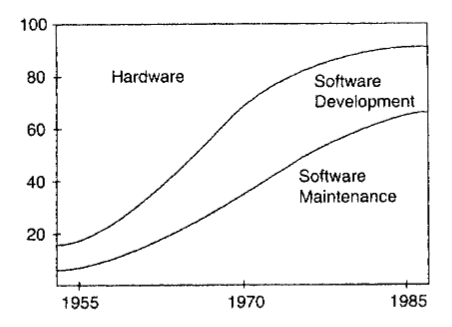
\includegraphics[width=0.4\textwidth]{img/Fig1.1.png}
    \caption{Costo de mantenimiento vs costo de desarrollo.}
    \label{fig:maint}
\end{figure}

\begin{mydef}{}{}
    El mantenimiento \textbf{correctivo} se refiere a la eliminación de errores residuales o \textit{bugs} que se descubren una vez que el software ha sido entregado y desplegado. Implica la eliminación de defectos que causan que el software se comporte de manera inconsistente con sus requisitos o necesidades del cliente.
\end{mydef}

\begin{mydef}{}{}
    El mantenimiento \textbf{adaptativo} se realiza para mejorar funcionalmente el software (conocidos como "upgrades") o para adaptarlo a los cambios en su entorno. También abarca la adición de nuevas funcionalidades o características que no estaban presentes en la versión original, a menudo impulsadas por la evolución de las necesidades del negocio o la aparición de nuevas tecnologías.
\end{mydef}


\section{Enfoque de la Ingeniería en Software}

En gran medida, el proceso de software determina la calidad del producto y la productividad alcanzada. Por lo tanto, para abordar el dominio del problema y enfrentar con éxito los desafíos de la ingeniería de software, es necesario centrarse en el proceso de software. El diseño de procesos adecuados y su control se convierten así en un objetivo clave de la investigación en ingeniería de software.

\subsection{El proceso de desarrollo en fases}

\begin{itemize}
    \item Cada fase termina con una \textbf{salida definida}.
    \item Las fases se realizan en el \textbf{orden especificado} por el modelo de proceso que se elija seguir.
    \item El motivo de separar en fases es la \textbf{separación de incumbencias}: cada fase manipula distintos aspectos del desarrollo de software.
    \item El proceso en fases permite \textbf{verificar la calidad y progreso} en momentos definidos del desarrollo, al final de la fase.
\end{itemize}

En general, las fases son:
\begin{itemize}
    \item \underline{\textbf{Análisis y especificación de requerimientos}}.
    \item \underline{\textbf{Arquitectura}}.
    \item \underline{\textbf{Diseño}}.
    \item \underline{\textbf{Codificación}}
    \item \underline{\textbf{Testing}}.
    \item \underline{\textbf{Entrega e instalación}}.
\end{itemize}

\newpage

\section{Análisis y especificación de requerimientos}